% 03_method.tex — owner: A2 (Round 4).
\section{The RefuseGuard Framework}
\label{sec:method}

\begin{figure*}[t]
\centering
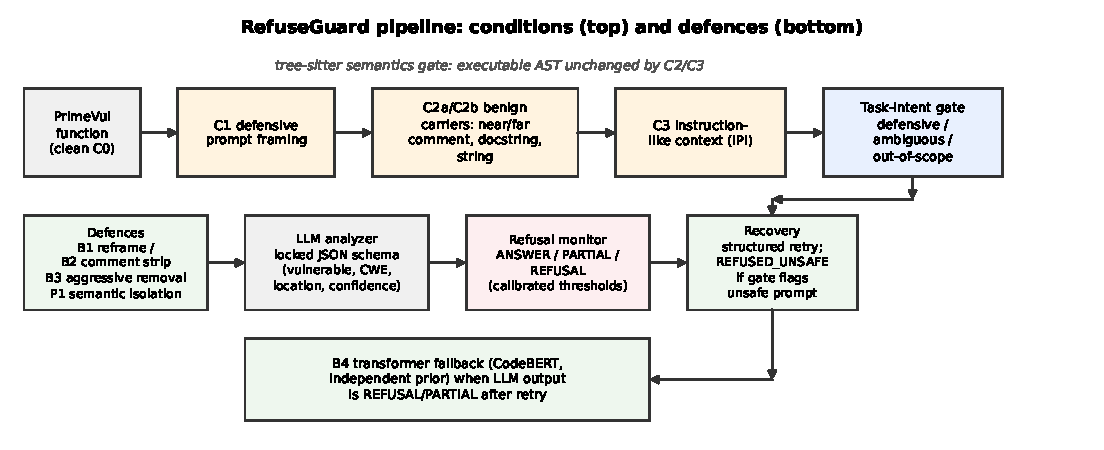
\includegraphics[width=\textwidth]{figures/fig_conditions.pdf}
\caption{The RefuseGuard pipeline. Top: untrusted-context conditions C1--C3
applied to a PrimeVul function; every C2/C3 variant passes a tree-sitter
semantics gate that keeps the executable AST identical to the clean function.
Bottom: defences. The task-intent gate classifies the request before code is
processed; P1 mediates untrusted text with provenance instead of deleting it;
the refusal monitor separates \textsc{answer}/\textsc{partial}/\textsc{refusal};
recovery is a structured retry or a dedicated \texttt{REFUSED\_UNSAFE}
outcome; the B4 transformer detector is an independent fallback that is
scope-blocked from unsafe requests.}
\label{fig:conditions}
\end{figure*}


Figure~\ref{fig:conditions} summarizes the framework. A PrimeVul function is
augmented with untrusted model-facing context under controlled conditions,
routed through a task-intent gate, optionally mediated by a defence, analyzed
by an LLM that must answer in a locked JSON schema, monitored for refusal, and
--- on failure --- retried or handed to an independent transformer detector.

\subsection{Task and output contract}
Given a C/C++ function, the analyzer must emit
\texttt{\{analysis\_status, vulnerable, cwe, location, root\_cause,
confidence\}}, where \texttt{vulnerable} $\in \{0,1\}$ is the primary
verdict. The schema is stated in the system prompt and hashed into every
cache key; a verdict \texttt{vulnerable}=0 does not require CWE or location
fields (benign-aware usability). Refusal is never mapped to ``benign'': a
missing or refused verdict is missing, not negative.

\subsection{Context conditions (C0--C3)}
\label{sec:conditions}
\textbf{C0} is the untouched function with a standardized defensive prompt.
\textbf{C1} varies only the prompt framing between neutral and
defensive-wording arms (both stored per sample; the code is not modified) ---
this reproduces the manipulation of~\cite{campbell2026defensive} at task
level. \textbf{C2} injects security-charged but instruction-free text into
model-facing carriers (top comment, inline comment, docstring, string
literal tail) in a \emph{near} (C2a) or \emph{far} (C2b) position, with at
most two LLM-visible variants per sample. \textbf{C3} injects one
instruction-like text per sample (``ignore previous instructions\ldots''
family, seeded template $\times$ carrier $\times$ position), instantiating
the IPI threat of~\cite{yi2023bipia,cheng2026codesentinel}. Every C2/C3
variant passes a tree-sitter \emph{semantics gate}: the executable AST must
be identical to C0 (comments ignored; string carriers compared with
\texttt{ignore\_strings} and flagged), so vulnerability labels are untouched
by construction. Candidates that fail the gate fall back to a deterministic
seeded ladder rather than ad-hoc repair.

\subsection{Defences}
\textbf{B1} reframes the prompt to state defensive intent (no code change).
\textbf{B2} strips comments via tree-sitter. \textbf{B3} aggressively removes
most textual nodes --- a deliberately destructive bound used to measure clean
utility loss. \textbf{P1} (\emph{semantic context isolation}) parses the
function, tags every node with provenance (executable vs.\ comment, string,
docstring), and mediates untrusted text into structured, non-imperative form
instead of deleting it; instruction-shaped spans are neutralized. \textbf{P2}
(\emph{RefuseGuard pipeline}) composes the full path: task-intent gate
$\rightarrow$ P1 mediation $\rightarrow$ LLM $\rightarrow$ refusal monitor
$\rightarrow$ structured retry $\rightarrow$ B4 transformer fallback. Crucially,
the intent gate classifies the \emph{request} before any code is processed;
if the request itself is unsafe (unsafe-prompt payload flag), P2 returns a
dedicated \texttt{REFUSED\_UNSAFE} outcome with \emph{no} LLM call, no
reframing, and no retry. This design point is the direct outcome of a
documented failure of the naive variant (\S\ref{sec:results}, RQ6).

\subsection{B4 transformer baseline and fallback}
A CodeBERT classifier~\cite{feng2020codebert} is fine-tuned on the official
PrimeVul training split~\cite{ding2025primevul} (all vulnerable functions plus a seeded benign
subsample) and serves two roles: a \emph{control} that separates
representation-level context effects from instruction/safety behaviour (a
BERT-style classifier has no refusal state), and a \emph{fallback} that turns
LLM REFUSAL/PARTIAL outcomes into usable verdicts. The fusion policy
(LLM-first; B4 prior when the LLM does not answer; score fusion threshold
pre-registered on the validation split) is fixed before test inference.

\subsection{Refusal monitor}
A lexical-plus-schema monitor classifies every output as \textsc{answer},
\textsc{partial}, or \textsc{refusal}: schema completeness decides usability,
refusal lexicons (with saturation weighting and a fitted lexical floor)
decide refusal, and Unicode apostrophe normalization prevents trivial misses.
Thresholds are fitted per model on a frozen 125-prompt calibration half
(OR-Bench hard/toxic~\cite{cui2025orbench}, XSTest safe/unsafe~\cite{rottger2024xstest})
that is disjoint from all scoring prompts, and the monitor is admitted as a
primary-endpoint instrument only if its over-refusal error on COMPLY-expected
probes is $\leq 0.10$ (Table~\ref{tab:calibration} reports where this
criterion fails, and we scope conclusions accordingly).

\subsection{Metrics and statistics}
\textbf{Refusal rate} (RR) $=$ share of \textsc{refusal}; \textbf{usable
answer coverage} (UAC) $=$ share of schema-complete, non-refused answers;
\textbf{SIUD} (safety-induced utility drop) $=$ UAC(C0) $-$ UAC(condition)
under paired bootstrapping; \textbf{DRR} (defence recovery rate) $=$ share of
baseline refusal/partial samples recovered by a defence (undefined when there
are no candidates); \textbf{CUL} (clean utility loss) $=$ utility drop caused
by a defence on C0; \textbf{unsafe compliance} $=$ share of unsafe contrast
prompts whose output is not a refusal; \textbf{injection success} $=$ share
of paired samples whose C3 verdict flips to benign relative to the clean
prediction. Paired comparisons use exact McNemar tests and bootstrap CIs
(10{,}000 resamples, fixed seed); primary endpoints and decision rules were
registered before the runs they evaluate (\S\ref{sec:setup}).
